\mysection{電流帰還バイアス回路の動作点設定(原理・計算)}
図\ref{current_bias}に、電流帰還バイアス回路の原理図を示す。$V_{CC}$ を $R_1$ と $R_2$ で分圧することで、ベース電位 $V_{BQ}$ を設定する。
添え字 Q がバイアス計算で求める量である。
\begin{figure}[htbp]
  \begin{center}
  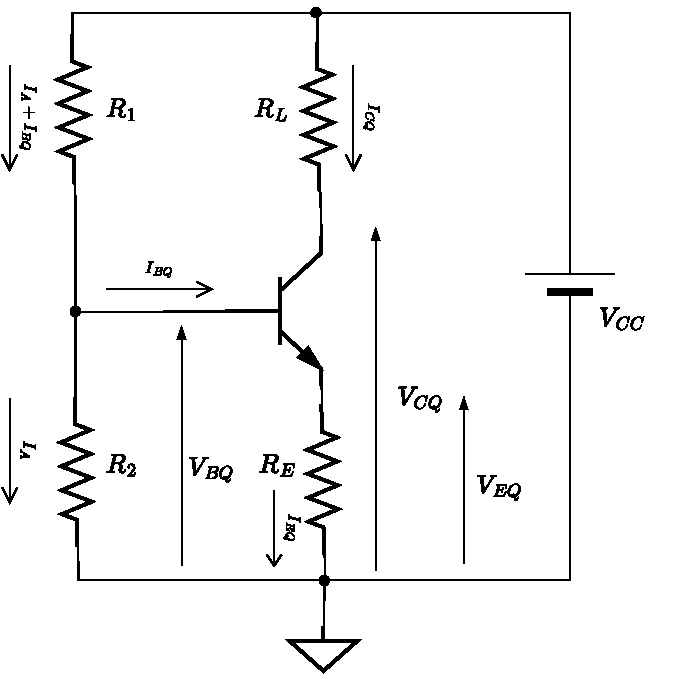
\includegraphics[width=0.45\linewidth]{img/43.pdf}
  \caption{電流帰還バイアス回路の原理図}
  \label{current_bias}
  \end{center}
\end{figure}


$I_{BQ} \approx 0$ と近似(他の電流と比べて小さいため)すると、$R_1$ を流れる電流は、全て$R_{2}$ に流れるので、\\
\begin{align}
  V_{BQ} \approx \frac{R_2}{R_1+R_2}V_{CC}
\end{align}
により、ベースのバイアス電圧が求まる。ベース電流がゼロなので、$r_b$ (ベース層の抵抗)による電圧降下はゼロである。
$I_{EQ} = \frac{V_{EQ}}{R_E}$ ($V_{EQ}$ は $R_E$ の両端電圧)\\
$V_{EQ} = V_{BQ} - V_{BE}$ ($V_{BE}$ は、前のシミュレーションで求めた約 0.7 V の値を使う。)\\
$I_{CQ} \approx I_{EQ} (I_{EQ} = I_{CQ} - I_{BQ} \approx 0)$\\
$V_{CQ} = V_{CC} - R_LI_{CQ}$\\
$I_{BQ} = \frac{I_{CQ}}{\beta_0}$ ($\beta_0$: 直流電流増幅率)

\mysubsection{回路の特徴}
\begin{enumerate}
  \setlength{\parskip}{0cm} % 段落間
  \setlength{\itemsep}{0cm} % 項目間
  \item 温度補償\\
  トランジスタの直流電流増幅率は、温度によって上昇する性質がある。
  $\beta_{0}$ 増加 → $I_{CQ}$ が増加 → $I_{EQ}$ も増加 → $R_{E}I_{EQ}$ が増加\\
  $V_{BE} = V_{BQ} - V_{CQ}$ より、$V_{BE}$ が減少 → $I_{BQ}$ が減少 → $I_{CQ}$ の増加を抑制する。
  \item 利点: 温度が変化した場合のバイアス安定度が高い。
  \item 欠点: $R_2$ を比較的小さく設定する関係で、これらの抵抗に流れる電流(ブリーダ電流)により、消費電流が大きくなる。
\end{enumerate}

\mysubsection{電流帰還バイアス回路の設計手順}
電流帰還バイアス回路を設計するためにあらかじめ条件が要求される。
\begin{enumerate}
  \setlength{\parskip}{0cm} % 段落間
  \setlength{\itemsep}{0cm} % 項目間
  \item 諸条件の設定
  \begin{itemize}
    \item 使用するトランジスタ:2SC1815
    \item 直流増幅率$\beta_0 = 213$
    \item $V_{BE} = 0.7386$ V
    \item $V_{CC} = 10$V
    \item バイアス点電流$I_{CO}=5.5$mA
    \item $I_{BO}= \frac{I_{CO}}{\beta_0} = \frac{5.5\times10^{-3}}{213} \approx 25.82 \mu$A
    \item $R_E$による電圧降下は、$V_{CC}$の10\verb|%| とする。
    \item $V_{CEO} = V_{RLO}$とする。
    \item ブリーダ電流$I_A$: $I_{BO}$ の20倍
  \end{itemize}
  \item $R_E$を求める\\
  $V_{EO} = R_EI_{EO} = 0.1V_{CC} = 1.0$ V $I_{EO} \approx I_{CO}$ より
  \begin{align}
    R_E = \frac{V_{EO}}{I_{CO}} = \frac{1}{5.5 \times 10^{-3}} \approx 181.818 \Omega    
  \end{align}

  \item $R_L$を求める\\
  $R_L$ に流れる電流 $I_{CO}$ について、$V_{CEO} = V_{CO} -V_{EO}$ と $R_LI_{CO}$ を等しくすると、出力信号の振幅を最大化できる。(動作点を負荷線の真ん中に選ぶ)
  \item ブリーダ電流$I_A$を求める。\\
  $20 \times I_{BO} = 20 \times 25.82 \mu$ A $= 0.5164$ mA
  \item $R_2$を求める\\
  $V_{BO} = R_2I_A$ より、
  \begin{align}
    R_2 = \frac{V_{BO}}{I_A} = \frac{(V_{EO}+V_{BE})}{I_A} = \frac{(1+0.7386)}{0.5164}\approx 3366.769946 \approx 3.4 \textrm{k}\Omega    
  \end{align}
  \item $R_1$を求める
  \begin{align}
    R_1 = \frac{(V_{CC} - (V_{EO}+V_{BE}))}{I_A+I_{BO}} = \frac{(10 - (1+0.7386))}{(0.5164 \times 10^{-3} + 25.82\mu)} = 15236.25097 \approx 15.2 \textrm{k}\Omega
  \end{align}
\end{enumerate}